% fig_schematic_rudder.tex — Lazy Rudder conceptual schematic (TikZ).
% \input-ted inside a figure environment in main.tex.
% Requires: \usepackage{tikz} in preamble.
%
% Diagram: 2D representation of the pretrained singular-vector cone.
%  - Gray shaded ellipse = base pretrained subspace (top-k cone).
%  - Hatched region outside ellipse = orthogonal complement (dominates absolute mass).
%  - Black arrow along cone axis = base pretrained "flow" (dominant singular vectors).
%  - Small red arrow near axis = alignment rudder Delta W (deflection, srank ~ 3-4 dims).
%  - Labeled singular vectors (v1, v2) as thin gray arrows inside cone.

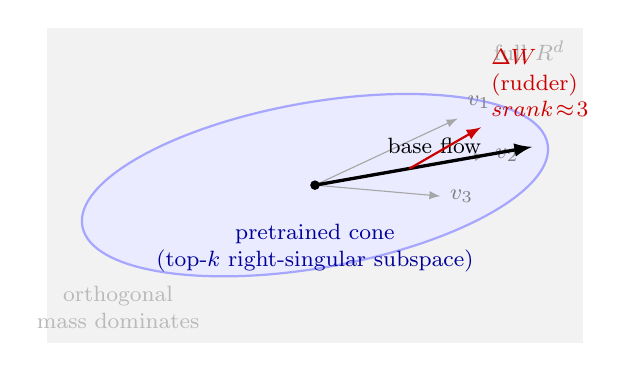
\begin{tikzpicture}[
  >=latex,
  font=\small,
  flow/.style={very thick, ->, black},
  rudder/.style={thick, ->, red!80!black},
  svec/.style={thin, ->, gray!70},
  baseline=(current bounding box.center)
]

% ── outer box (full parameter space) ────────────────────────────────────────
\fill[gray!10] (-3.4,-2.0) rectangle (3.4,2.0);
\node[gray!60, anchor=north east] at (3.3,1.95) {\footnotesize full $\mathbb{R}^{d}$};

% ── pretrained cone (ellipse) ────────────────────────────────────────────────
\begin{scope}
  \clip (-3.4,-2.0) rectangle (3.4,2.0);
  \fill[blue!8, rotate=10] (0,0) ellipse (3.0cm and 1.05cm);
  \draw[blue!35, thick, rotate=10] (0,0) ellipse (3.0cm and 1.05cm);
\end{scope}

% ── orthogonal-complement hatching label ─────────────────────────────────────
\node[gray!55, align=center, font=\footnotesize] at (-2.5, -1.55)
  {orthogonal\\mass dominates};

% ── singular vector arrows inside cone ───────────────────────────────────────
\draw[svec] (0,0) -- ++(25:2.0)  node[above right, gray, font=\footnotesize] {$v_1$};
\draw[svec] (0,0) -- ++(10:2.2)  node[right,       gray, font=\footnotesize] {$v_2$};
\draw[svec] (0,0) -- ++(-5:1.6)  node[right,       gray, font=\footnotesize] {$v_3$};

% ── base flow (dominant direction) ───────────────────────────────────────────
\draw[flow] (0,0) -- ++(10:2.8)
  node[pos=0.55, above, font=\footnotesize, black] {base flow};

% ── alignment rudder (small deflection) ──────────────────────────────────────
\draw[rudder] (1.2, 0.21) -- ++(30:1.05)
  node[above right, font=\footnotesize, red!80!black, align=left]
    {$\Delta W$\\(rudder)\\$srank\!\approx\!3$};

% ── cone label ───────────────────────────────────────────────────────────────
\node[blue!60!black, font=\footnotesize, align=center] at (0, -0.8)
  {pretrained cone\\(top-$k$ right-singular subspace)};

% ── origin dot ───────────────────────────────────────────────────────────────
\filldraw[black] (0,0) circle (1.5pt);

\end{tikzpicture}
